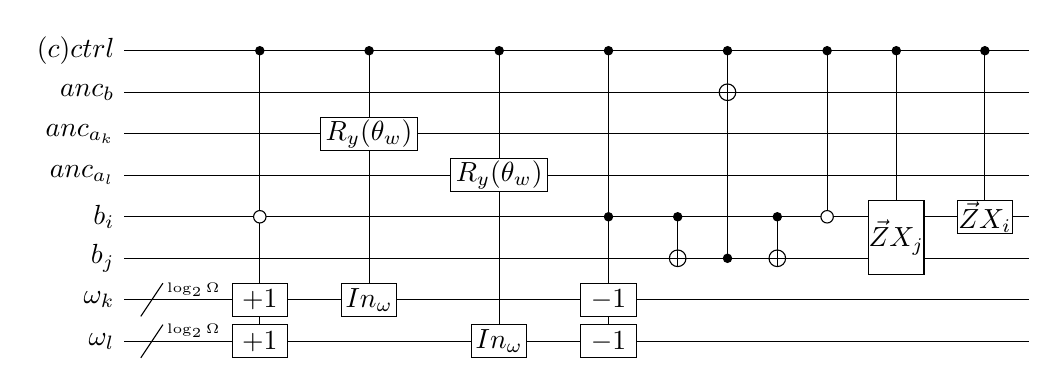
\begin{tikzpicture}[scale=1.000000,x=1pt,y=1pt]
\filldraw[color=white] (0.000000, -7.500000) rectangle (327.000000, 112.500000);
% Drawing wires
% Line 1: ctrl W \text{(c) }ctrl
\draw[color=black] (0.000000,105.000000) -- (327.000000,105.000000);
\draw[color=black] (0.000000,105.000000) node[left] {$\text{(c) }ctrl$};
% Line 2: anc_b W anc_b
\draw[color=black] (0.000000,90.000000) -- (327.000000,90.000000);
\draw[color=black] (0.000000,90.000000) node[left] {$anc_b$};
% Line 3: anc_k W anc_{a_k}
\draw[color=black] (0.000000,75.000000) -- (327.000000,75.000000);
\draw[color=black] (0.000000,75.000000) node[left] {$anc_{a_k}$};
% Line 4: anc_l W anc_{a_l}
\draw[color=black] (0.000000,60.000000) -- (327.000000,60.000000);
\draw[color=black] (0.000000,60.000000) node[left] {$anc_{a_l}$};
% Line 5: i W b_i
\draw[color=black] (0.000000,45.000000) -- (327.000000,45.000000);
\draw[color=black] (0.000000,45.000000) node[left] {$b_i$};
% Line 6: j W b_j
\draw[color=black] (0.000000,30.000000) -- (327.000000,30.000000);
\draw[color=black] (0.000000,30.000000) node[left] {$b_j$};
% Line 7: k W \omega_k
\draw[color=black] (0.000000,15.000000) -- (327.000000,15.000000);
\draw[color=black] (0.000000,15.000000) node[left] {$\omega_k$};
% Line 8: l W \omega_l
\draw[color=black] (0.000000,0.000000) -- (327.000000,0.000000);
\draw[color=black] (0.000000,0.000000) node[left] {$\omega_l$};
% Done with wires; drawing gates
% Line 10: k / ^{\log_2{\Omega}}
\draw (6.000000, 9.000000) -- (14.000000, 21.000000);
\draw (12.000000, 18.000000) node[right] {$\scriptstyle{^{\log_2{\Omega}}}$};
% Line 11: l / ^{\log_2{\Omega}}
\draw (6.000000, -6.000000) -- (14.000000, 6.000000);
\draw (12.000000, 3.000000) node[right] {$\scriptstyle{^{\log_2{\Omega}}}$};
% Line 12: ctrl i j anc_b anc_k anc_l k l LABEL width=1
% Line 14: k G width=20 $+1$ l G width=20 $+1$ ctrl -i
\draw (49.000000,105.000000) -- (49.000000,0.000000);
\begin{scope}
\draw[fill=white] (49.000000, 15.000000) +(-45.000000:14.142136pt and 8.485281pt) -- +(45.000000:14.142136pt and 8.485281pt) -- +(135.000000:14.142136pt and 8.485281pt) -- +(225.000000:14.142136pt and 8.485281pt) -- cycle;
\clip (49.000000, 15.000000) +(-45.000000:14.142136pt and 8.485281pt) -- +(45.000000:14.142136pt and 8.485281pt) -- +(135.000000:14.142136pt and 8.485281pt) -- +(225.000000:14.142136pt and 8.485281pt) -- cycle;
\draw (49.000000, 15.000000) node {$+1$};
\end{scope}
\begin{scope}
\draw[fill=white] (49.000000, -0.000000) +(-45.000000:14.142136pt and 8.485281pt) -- +(45.000000:14.142136pt and 8.485281pt) -- +(135.000000:14.142136pt and 8.485281pt) -- +(225.000000:14.142136pt and 8.485281pt) -- cycle;
\clip (49.000000, -0.000000) +(-45.000000:14.142136pt and 8.485281pt) -- +(45.000000:14.142136pt and 8.485281pt) -- +(135.000000:14.142136pt and 8.485281pt) -- +(225.000000:14.142136pt and 8.485281pt) -- cycle;
\draw (49.000000, -0.000000) node {$+1$};
\end{scope}
\filldraw (49.000000, 105.000000) circle(1.500000pt);
\draw[fill=white] (49.000000, 45.000000) circle(2.250000pt);
% Line 15: anc_k G:width=35 $R_y(\theta_w)$ k G:width=20 $In_\omega$ ctrl
\draw (88.500000,105.000000) -- (88.500000,15.000000);
\begin{scope}
\draw[fill=white] (88.500000, 75.000000) +(-45.000000:24.748737pt and 8.485281pt) -- +(45.000000:24.748737pt and 8.485281pt) -- +(135.000000:24.748737pt and 8.485281pt) -- +(225.000000:24.748737pt and 8.485281pt) -- cycle;
\clip (88.500000, 75.000000) +(-45.000000:24.748737pt and 8.485281pt) -- +(45.000000:24.748737pt and 8.485281pt) -- +(135.000000:24.748737pt and 8.485281pt) -- +(225.000000:24.748737pt and 8.485281pt) -- cycle;
\draw (88.500000, 75.000000) node {$R_y(\theta_w)$};
\end{scope}
\begin{scope}
\draw[fill=white] (88.500000, 15.000000) +(-45.000000:14.142136pt and 8.485281pt) -- +(45.000000:14.142136pt and 8.485281pt) -- +(135.000000:14.142136pt and 8.485281pt) -- +(225.000000:14.142136pt and 8.485281pt) -- cycle;
\clip (88.500000, 15.000000) +(-45.000000:14.142136pt and 8.485281pt) -- +(45.000000:14.142136pt and 8.485281pt) -- +(135.000000:14.142136pt and 8.485281pt) -- +(225.000000:14.142136pt and 8.485281pt) -- cycle;
\draw (88.500000, 15.000000) node {$In_\omega$};
\end{scope}
\filldraw (88.500000, 105.000000) circle(1.500000pt);
% Line 16: anc_l G:width=35 $R_y(\theta_w)$ l G:width=20 $In_\omega$ ctrl
\draw (135.500000,105.000000) -- (135.500000,0.000000);
\begin{scope}
\draw[fill=white] (135.500000, 60.000000) +(-45.000000:24.748737pt and 8.485281pt) -- +(45.000000:24.748737pt and 8.485281pt) -- +(135.000000:24.748737pt and 8.485281pt) -- +(225.000000:24.748737pt and 8.485281pt) -- cycle;
\clip (135.500000, 60.000000) +(-45.000000:24.748737pt and 8.485281pt) -- +(45.000000:24.748737pt and 8.485281pt) -- +(135.000000:24.748737pt and 8.485281pt) -- +(225.000000:24.748737pt and 8.485281pt) -- cycle;
\draw (135.500000, 60.000000) node {$R_y(\theta_w)$};
\end{scope}
\begin{scope}
\draw[fill=white] (135.500000, -0.000000) +(-45.000000:14.142136pt and 8.485281pt) -- +(45.000000:14.142136pt and 8.485281pt) -- +(135.000000:14.142136pt and 8.485281pt) -- +(225.000000:14.142136pt and 8.485281pt) -- cycle;
\clip (135.500000, -0.000000) +(-45.000000:14.142136pt and 8.485281pt) -- +(45.000000:14.142136pt and 8.485281pt) -- +(135.000000:14.142136pt and 8.485281pt) -- +(225.000000:14.142136pt and 8.485281pt) -- cycle;
\draw (135.500000, -0.000000) node {$In_\omega$};
\end{scope}
\filldraw (135.500000, 105.000000) circle(1.500000pt);
% Line 17: k G width=20 $-1$ l G width=20 $-1$ ctrl i
\draw (175.000000,105.000000) -- (175.000000,0.000000);
\begin{scope}
\draw[fill=white] (175.000000, 15.000000) +(-45.000000:14.142136pt and 8.485281pt) -- +(45.000000:14.142136pt and 8.485281pt) -- +(135.000000:14.142136pt and 8.485281pt) -- +(225.000000:14.142136pt and 8.485281pt) -- cycle;
\clip (175.000000, 15.000000) +(-45.000000:14.142136pt and 8.485281pt) -- +(45.000000:14.142136pt and 8.485281pt) -- +(135.000000:14.142136pt and 8.485281pt) -- +(225.000000:14.142136pt and 8.485281pt) -- cycle;
\draw (175.000000, 15.000000) node {$-1$};
\end{scope}
\begin{scope}
\draw[fill=white] (175.000000, -0.000000) +(-45.000000:14.142136pt and 8.485281pt) -- +(45.000000:14.142136pt and 8.485281pt) -- +(135.000000:14.142136pt and 8.485281pt) -- +(225.000000:14.142136pt and 8.485281pt) -- cycle;
\clip (175.000000, -0.000000) +(-45.000000:14.142136pt and 8.485281pt) -- +(45.000000:14.142136pt and 8.485281pt) -- +(135.000000:14.142136pt and 8.485281pt) -- +(225.000000:14.142136pt and 8.485281pt) -- cycle;
\draw (175.000000, -0.000000) node {$-1$};
\end{scope}
\filldraw (175.000000, 105.000000) circle(1.500000pt);
\filldraw (175.000000, 45.000000) circle(1.500000pt);
% Line 19: i +j
\draw (200.000000,45.000000) -- (200.000000,30.000000);
\filldraw (200.000000, 45.000000) circle(1.500000pt);
\begin{scope}
\draw[fill=white] (200.000000, 30.000000) circle(3.000000pt);
\clip (200.000000, 30.000000) circle(3.000000pt);
\draw (197.000000, 30.000000) -- (203.000000, 30.000000);
\draw (200.000000, 27.000000) -- (200.000000, 33.000000);
\end{scope}
% Line 20: ctrl j +anc_b
\draw (218.000000,105.000000) -- (218.000000,30.000000);
\filldraw (218.000000, 105.000000) circle(1.500000pt);
\filldraw (218.000000, 30.000000) circle(1.500000pt);
\begin{scope}
\draw[fill=white] (218.000000, 90.000000) circle(3.000000pt);
\clip (218.000000, 90.000000) circle(3.000000pt);
\draw (215.000000, 90.000000) -- (221.000000, 90.000000);
\draw (218.000000, 87.000000) -- (218.000000, 93.000000);
\end{scope}
% Line 21: i +j
\draw (236.000000,45.000000) -- (236.000000,30.000000);
\filldraw (236.000000, 45.000000) circle(1.500000pt);
\begin{scope}
\draw[fill=white] (236.000000, 30.000000) circle(3.000000pt);
\clip (236.000000, 30.000000) circle(3.000000pt);
\draw (233.000000, 30.000000) -- (239.000000, 30.000000);
\draw (236.000000, 27.000000) -- (236.000000, 33.000000);
\end{scope}
% Line 23: ctrl -i
\draw (254.000000,105.000000) -- (254.000000,45.000000);
\filldraw (254.000000, 105.000000) circle(1.500000pt);
\draw[fill=white] (254.000000, 45.000000) circle(2.250000pt);
% Line 25: i j G width=20 $\vec{Z}X_j$ ctrl
\draw (279.000000,105.000000) -- (279.000000,30.000000);
\begin{scope}
\draw[fill=white] (279.000000, 37.500000) +(-45.000000:14.142136pt and 19.091883pt) -- +(45.000000:14.142136pt and 19.091883pt) -- +(135.000000:14.142136pt and 19.091883pt) -- +(225.000000:14.142136pt and 19.091883pt) -- cycle;
\clip (279.000000, 37.500000) +(-45.000000:14.142136pt and 19.091883pt) -- +(45.000000:14.142136pt and 19.091883pt) -- +(135.000000:14.142136pt and 19.091883pt) -- +(225.000000:14.142136pt and 19.091883pt) -- cycle;
\draw (279.000000, 37.500000) node {$\vec{Z}X_j$};
\end{scope}
\filldraw (279.000000, 105.000000) circle(1.500000pt);
% Line 26: i G width=20 $\vec{Z}X_i$ ctrl
\draw (311.000000,105.000000) -- (311.000000,45.000000);
\begin{scope}
\draw[fill=white] (311.000000, 45.000000) +(-45.000000:14.142136pt and 8.485281pt) -- +(45.000000:14.142136pt and 8.485281pt) -- +(135.000000:14.142136pt and 8.485281pt) -- +(225.000000:14.142136pt and 8.485281pt) -- cycle;
\clip (311.000000, 45.000000) +(-45.000000:14.142136pt and 8.485281pt) -- +(45.000000:14.142136pt and 8.485281pt) -- +(135.000000:14.142136pt and 8.485281pt) -- +(225.000000:14.142136pt and 8.485281pt) -- cycle;
\draw (311.000000, 45.000000) node {$\vec{Z}X_i$};
\end{scope}
\filldraw (311.000000, 105.000000) circle(1.500000pt);
% Done with gates; drawing ending labels
% Done with ending labels; drawing cut lines and comments
% Done with comments
\end{tikzpicture}
